% L11b TJUL today: one panel, drawn to scale with numeric axes (instructor's choice,
% November 5, 2026). The profit at expiration (June 30, 2027), per share of SPY, of
% the collar that the Innovator Equity Defined Protection ETF (TJUL) holds, with
% SPY alone (gray, dashed) and the two options together (blue), as in the
% net debit panel of Fig-L11b-Collar. The SPY close on November 4, 2026 is marked
% in orange (the course's color for before expiration): the profit if SPY stayed
% at that price until expiration.
%
% Data (SEC Form N-PORT for TJUL, series S000080903, July 31, 2025; cost = value
% minus unrealized appreciation, per share = per contract / 100):
%   long put  K1 = 617.85 = S(0), the SPY close on June 30, 2025: P1 = 45.459
%   short call K2 = 701.94 = 617.85 x 1.1361 (the 13.61% cap):    P2 = 34.232
%   (the fund holds a call at 11.12 instead of the shares; the figure uses the
%   lecture's frame, shares bought at S(0))
% Growth to expiration: two-year Treasury yield on June 30, 2025 (FRED DGS2),
% 3.72%, semiannual bond-equivalent, so g_y = 2 ln(1 + 0.0372/2) = 0.03686/yr;
% T = 730/365 = 2 yr, D = exp(g_y T) = 1.07650.
%   net debit grown  D(P1 - P2)        = 12.086
%   cost grown       c = D(S0 + P1 - P2) = 677.202 (breakeven S-double-dagger)
%   SPY alone        S - D S0 = S - 665.117
%   collar: floor K1 - c = -59.352; S - c between the strikes; cap K2 - c = 24.738
%   options together: (K1 - S)^+ - (S - K2)^+ - 12.086, zero at K1 - 12.086 = 605.764,
%     where SPY alone crosses the floor and the opportunity loss starts
%   today, S = 766.81: SPY alone 101.693, collar 24.738, gap 76.956
% As in the net debit panel, no O+ is drawn: it is not where the loss starts.
%
% Coordinates: inside the data scope, x is SPY in USD (570 at the y-axis, 30 USD
% per 0.8 cm) and y is profit in USD/share (-100 at the x-axis, 35 USD per 0.8 cm).
\documentclass[tikz,border=4pt]{standalone}
% Shared style for the L11b profit diagrams (copied from L11a/figs on November 4, 2026), \input by each Fig-L11b-*.tex.
%
% Drawn on October 23, 2026 in the style of the CHEME 5800 L9c convexity and
% gradient-descent schematics: arrowed axes, a thick ink curve (the profit), a
% blue companion curve (the payoff), open circle markers, and dashed drops to
% colored axis labels. Each figure has two panels; each panel is a schematic,
% so the axes carry no numbers.
%
% Panel coordinates: x is the share price at expiration S(T), with the y-axis
% at S(T) = 0. Inside \begin{profitdata} ... \end{profitdata} the y coordinate
% is the profit (USD/share): the scope shifts the zero-profit line up to
% \yzero and scales profits by \yscale, so every path is written in the
% structure's own units. Nodes are not scaled.
%
% Math uses the standard TeX fonts (no unicode-math), as in the L9c figures,
% so S, K, and the double dagger match the notebook's math.
%
% The notebook SVG carries a dark palette added by theme_svg.py; keep new
% colors in that script's mapping when changing the palette here.
\usepackage[no-math]{fontspec}
\IfFontExistsTF{Arial}{\setsansfont{Arial}}{\setsansfont{TeX Gyre Heros}}
\renewcommand{\familydefault}{\sfdefault}
\usepackage{amsmath,amssymb}
\usetikzlibrary{arrows.meta,calc}

% Same colors as the L9c figures.
\definecolor{vnink}{HTML}{202124}
\definecolor{gdblue}{HTML}{0091FF}
\definecolor{gdred}{HTML}{E02020}
\definecolor{gdgray}{HTML}{6D7278}
% The L9c simulated-annealing orange, used only for profits before expiration.
\definecolor{saorange}{HTML}{F08C00}

% Panel geometry (x units): the axes run to \xaxis and \yaxis, the zero-profit
% line sits at \yzero, and a profit of 1 USD/share is \yscale units tall.
\def\xaxis{9.6}
\def\yaxis{6.3}
\def\yzero{3.9}
\def\yscale{0.8}
\def\panelgap{10.6}

\tikzset{
  every picture/.append style={x=0.8cm, y=0.8cm, font=\sffamily\small, text=vnink},
  axis/.style={draw=vnink, line width=0.8pt, -{Latex[length=2.6mm, width=1.8mm]}},
  zero/.style={draw=gdgray, line width=0.5pt},
  profit/.style={draw=vnink, line width=1.6pt, line join=round},
  payoff/.style={draw=gdblue, line width=1.2pt, line join=round},
  more/.style={-{Latex[length=2.4mm, width=1.7mm]}},
  drop/.style={draw=gdgray, line width=0.8pt, dash pattern=on 3pt off 2pt},
  gap/.style={draw=vnink, line width=0.8pt,
    {Latex[length=1.8mm, width=1.3mm]}-{Latex[length=1.8mm, width=1.3mm]}},
  pt/.style={circle, fill=white, line width=1.0pt, inner sep=0pt, minimum size=2.4mm},
  note/.style={text=gdgray, font=\sffamily\footnotesize, align=center},
  % L11b: the profit of the shares alone, for comparison (gray, dashed)
  shares/.style={draw=gdgray, line width=1.0pt, dash pattern=on 5pt off 3pt},
}

% Axes, zero-profit line, the bold run-in title (#1), and the axis labels
% (#2 horizontal, #3 vertical).
\newcommand{\panelaxes}[3]{%
  \draw[zero] (0, \yzero) -- (\xaxis - 0.2, \yzero);
  \draw[axis] (-0.15, 0) -- (\xaxis, 0);
  \draw[axis] (0, -0.15) -- (0, \yaxis);
  \node[anchor=east, text=gdgray] at (-0.05, \yzero) {$0$};
  \node[anchor=north] at (\xaxis/2, -1.05) {#2};
  \node[rotate=90, anchor=south] at (-0.55, \yaxis/2) {#3};
  \node[anchor=south] at (\xaxis/2, \yaxis + 0.15) {#1};
}
% The expiration diagrams' frame.
\newcommand{\panelframe}[1]{%
  \panelaxes{#1}{Share price at expiration $S(T)$}{Payoff and profit (USD/share)}}

% Scope in which (S, profit) are the coordinates.
\newenvironment{profitdata}{\begin{scope}[shift={(0, \yzero)}, yscale=\yscale]}{\end{scope}}

% A strike: dashed drop from the profit kink (#1, #2) to the S(T) axis, with the
% strike symbol #3 and, below it, the leg written at that strike, #4.
\newcommand{\strike}[4]{%
  \draw[drop] (#1, #2) -- (#1, -\yzero/\yscale);
  \node[anchor=north, align=center, inner sep=1.5pt, text=gdgray]
    at (#1, -\yzero/\yscale - 0.08/\yscale)
    {#3\\[-1.5pt]{\footnotesize\color{vnink}#4}};}

% The share price when the trade opens, S(0): a short tick on the S(T) axis at
% #1, labeled just above the axis so it clears the strike labels below it. Added
% October 27, 2026, so students can see where the strikes sit relative to today's
% price (the time-decay figure marks S(0) the same way).
\newcommand{\entryprice}[1]{%
  \draw[draw=vnink, line width=0.8pt] (#1, -\yzero/\yscale) -- (#1, -\yzero/\yscale + 0.2/\yscale);
  \node[anchor=south, inner sep=1.5pt, text=gdgray] at (#1, -\yzero/\yscale + 0.2/\yscale) {$S(0)$};}

% A breakeven: open red circle on the zero line at #1, label #2 placed #3 of
% the circle (above left or above right), clear of the circle's outline.
\newcommand{\breakeven}[3]{%
  \node[pt, draw=gdred,
    label={[text=gdred, inner sep=0.5pt, label distance=2pt]#3:#2}] at (#1, 0) {};}

% Maximum profit: arrow at S = #1 from the payoff (zero) up to the profit #2.
% For a credit structure the gap is the credit, grown to expiration.
\newcommand{\maxprofit}[2]{%
  \draw[gap] (#1, 0.06) -- (#1, #2 - 0.06);
  \node[anchor=south, inner sep=4pt] at (#1, #2) {max profit $=$ credit};}

% Maximum loss: arrow at S = #1 from zero down to the profit #2 (negative),
% label anchored #3 (west puts it to the right of the arrow).
\newcommand{\maxloss}[3]{%
  \draw[gap] (#1, -0.06) -- (#1, #2 + 0.06);
  \node[anchor=#3, inner sep=4pt] at (#1, #2/2) {max loss};}

% L11b: a two-entry legend in the panel's upper-left corner, the one corner the
% share-based profits never draw into: the position's profit (ink, label #1) and
% the shares alone (gray, dashed).
\newcommand{\shareslegend}[1]{%
  \draw[profit] (0.45, \yaxis - 0.35) -- (1.25, \yaxis - 0.35);
  \node[anchor=west, inner sep=3pt] at (1.25, \yaxis - 0.35) {#1};
  \draw[shares] (0.45, \yaxis - 0.95) -- (1.25, \yaxis - 0.95);
  \node[anchor=west, inner sep=3pt, text=gdgray] at (1.25, \yaxis - 0.95) {shares alone};}

% The structure's outlook (#1), as in the lecture's composite-contract table, in
% the panel's upper-right corner, the one corner no structure draws into. Added
% October 28, 2026, at the instructor's request.
\newcommand{\outlook}[1]{%
  \node[anchor=north east, inner sep=2pt, font=\sffamily\footnotesize]
    at (\xaxis, \yaxis) {{\color{gdgray}Outlook:} #1};}

% A loss that keeps growing as S(T) rises: note with its lower-left corner at
% (#1, #2), placed above the descending profit line near its arrowhead.
\newcommand{\unlimited}[2]{%
  \node[note, anchor=south west, inner sep=0pt] at (#1, #2) {unlimited\\loss};}


% data scope: (S, profit) in USD; the axes' corner is (570, -100)
\newenvironment{tjuldata}{\begin{scope}[x=0.8cm/30, y=0.8cm/35, shift={(-570, 100)}]}{\end{scope}}

\begin{document}
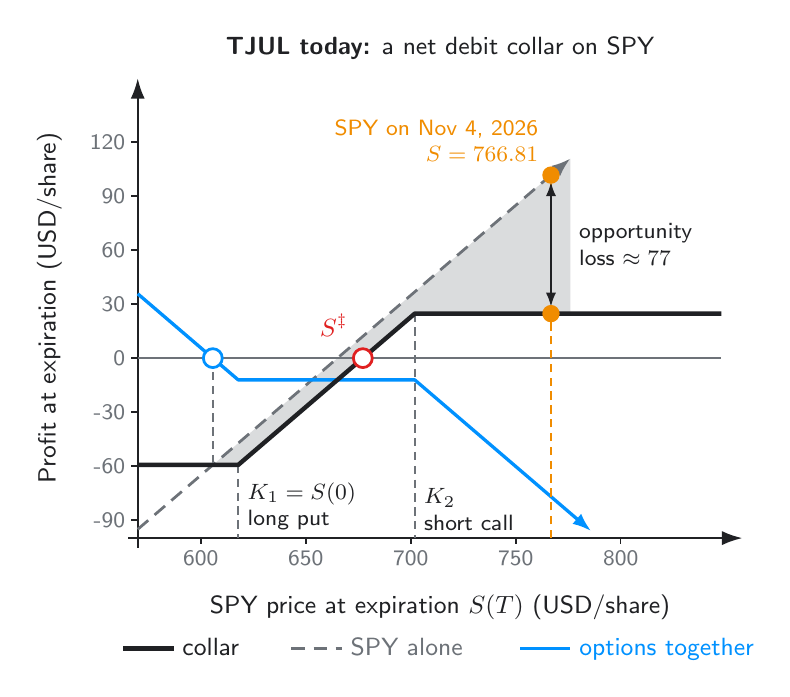
\begin{tikzpicture}
  % axes (panel units: 0.8 cm), title, axis labels
  \draw[axis] (-0.15, 0) -- (9.6, 0);
  \draw[axis] (0, -0.15) -- (0, 7.3);
  \node[anchor=south] at (4.8, 7.45) {\textbf{TJUL today:} a net debit collar on SPY};
  \node[rotate=90, anchor=south] at (-1.05, 3.65) {Profit at expiration (USD/share)};
  \node[anchor=north] at (4.8, -0.75) {SPY price at expiration $S(T)$ (USD/share)};
  \begin{tjuldata}
    % zero-profit line and tick marks with values
    \draw[zero] (570, 0) -- (848, 0);
    \foreach \s in {600, 650, 700, 750, 800}
      \draw[draw=vnink, line width=0.6pt] (\s, -100) -- ++(0, -3.5)
        node[below, inner sep=2pt, font=\sffamily\footnotesize, text=gdgray] {\s};
    \foreach \p in {-90, -60, -30, 0, 30, 60, 90, 120}
      \draw[draw=vnink, line width=0.6pt] (570, \p) -- ++(-3, 0)
        node[left, inner sep=2pt, font=\sffamily\footnotesize, text=gdgray] {\p};
    % opportunity loss: SPY alone above the collar, from the floor crossing to the
    % end of the SPY-alone line (S = 776, so its label fits to the right)
    \fill[gdgray, fill opacity=0.25] (605.764, -59.352) -- (776, 110.883)
      -- (776, 24.738) -- (701.94, 24.738) -- (617.85, -59.352) -- cycle;
    % strikes: drops from the collar's kinks to the axis, labeled inside the panel
    \draw[drop] (617.85, -59.352) -- (617.85, -100);
    \draw[drop] (701.94, 24.738) -- (701.94, -100);
    \node[anchor=south west, align=left, inner sep=2pt, font=\sffamily\footnotesize]
      at (619.5, -99) {$K_{1}=S(0)$\\long put};
    \node[anchor=south west, align=left, inner sep=2pt, font=\sffamily\footnotesize]
      at (703.5, -99) {$K_{2}$\\short call};
    % SPY alone, S - 665.117, from the y-axis to the end of the shading
    \draw[shares, more] (570, -95.117) -- (776, 110.883);
    % options together, drawn before the collar
    \draw[payoff, more] (570, 35.764) -- (617.85, -12.086) -- (701.94, -12.086) -- (786, -96.146);
    % collar
    \draw[profit] (570, -59.352) -- (617.85, -59.352) -- (701.94, 24.738) -- (848, 24.738);
    % breakeven
    % the label sits above the SPY-alone line, which crosses zero at 665.117 just
    % left of the circle; below it, the blue line at -12.086 leaves no room
    \node[pt, draw=gdred] at (677.202, 0) {};
    \node[anchor=south east, inner sep=0.5pt, text=gdred] at (671, 11) {$S^{\ddagger}$};
    % the options together break even where the loss starts: drop to the floor crossing
    \draw[drop] (605.764, 0) -- (605.764, -59.352);
    \node[pt, draw=gdblue] at (605.764, 0) {};
    % today: SPY close on November 4, 2026
    \draw[draw=saorange, line width=0.8pt, dash pattern=on 3pt off 2pt] (766.81, -100) -- (766.81, 101.693);
    \draw[gap] (766.81, 28.5) -- (766.81, 97.9);
    \node[anchor=west, align=left, inner sep=0pt, font=\sffamily\footnotesize] at (780, 63.2) {opportunity\\loss $\approx 77$};
    \node[circle, fill=saorange, inner sep=0pt, minimum size=2.2mm] at (766.81, 24.738) {};
    \node[circle, fill=saorange, inner sep=0pt, minimum size=2.2mm] at (766.81, 101.693) {};
    % above-left of the dot, clear of the SPY-alone line (below and right of it)
    \node[anchor=south east, align=right, inner sep=0pt, text=saorange, font=\sffamily\footnotesize] at (761, 109) {SPY on Nov 4, 2026\\$S=766.81$};
  \end{tjuldata}
  % legend: one row below the axis label (the upper-left corner holds today's label)
  \begin{scope}[shift={(4.8, -1.75)}]
    \draw[profit] (-5.03, 0) -- (-4.23, 0);
    \node[anchor=west, inner sep=3pt, text height=1.6ex, text depth=0.4ex] at (-4.23, 0) {collar};
    \draw[shares] (-2.36, 0) -- (-1.56, 0);
    \node[anchor=west, inner sep=3pt, text height=1.6ex, text depth=0.4ex, text=gdgray] at (-1.56, 0) {SPY alone};
    \draw[payoff] (1.27, 0) -- (2.07, 0);
    \node[anchor=west, inner sep=3pt, text height=1.6ex, text depth=0.4ex, text=gdblue] at (2.07, 0) {options together};
  \end{scope}
\end{tikzpicture}
\end{document}
